\documentclass[a4paper,onecolumn,11pt,unpublished]{quantumarticle}
\pdfoutput=1
\usepackage[T1]{fontenc}
\renewcommand{\rmdefault}{lmr}
\usepackage{amsmath,amssymb,booktabs,tabularx,graphicx,hyperref,minted,microtype}
\setminted{fontsize=\small,breaklines,tabsize=4,baselinestretch=1}
\setlength{\emergencystretch}{1.5em}
\usemintedstyle{friendly}
\newcommand{\C}{\mathbb C}
\newcommand{\B}{\mathbb B}
\newcommand{\Tr}{\operatorname{Tr}}
\newcommand{\ket}[1]{\lvert #1\rangle}
\newcommand{\bra}[1]{\langle #1\rvert}
\newcommand{\id}{\mathrm{id}}
\DeclareMathOperator{\diag}{diag}
\hypersetup{pdftitle={Qubit-as-a-Function},pdfauthor={Brian Mingus},pdfsubject={Quantum states, programming languages and semantics}}
\begin{document}
\title{Qubit-as-a-Function}
\author{Brian Mingus}
\affiliation{Cognatory, LLC}
\email{brian@cognatory.com}
\email{fqubit@gmail.com}
\date{8 November 2026}
\maketitle
\begin{abstract}
What can it mean to call a qubit a function? In a fixed basis the amplitudes of a pure qubit form a function on two labels. For a possibly mixed qubit, its probability of accepting each effect is a second, operationally complete function. We give the inverse in both cases and identify the equivalences, domains and dimensions on which the claims depend. A register wavefunction splits recursively by prefix even when its qubits are entangled. The splitting does not assign independent wavefunctions to its parts. We connect these facts to a century of work on state representations, quantum computation and higher-order processes. We implement QAF, a TatSu language whose runtime function values refer to physical wires. A function can be probed or coherently invoked with a specified pair of target operations. The implementation includes class methods, recursion, circuit construction, channels, instruments, native CUDA execution, a CPU reference and bounded provider translations. Lean checks the coordinate and prefix isomorphisms and a reversible translation of concrete source trees. A hosted Rigetti simulator returned 49 outcomes of 00 and 51 of 11 in 100 trials of a translated Bell circuit. We distinguish this experiment from the algebraic guarantee on its ideal program.
\end{abstract}
\section{The question at one wire}
Prepare a control in $\ket{+}=(\ket0+\ket1)/\sqrt2$ and a target in $\ket0$. Ask the control to select the identity or a bit flip on the target. In QAF the selector is a qubit that can subsequently be probed by another expression.
\inputminted{qaf}{../../examples/prefix/callable.qaf}
The joint computational probabilities are $(1/2,0,0,1/2)$. The last line asks for the probability of the $+1$ outcome of an $X$ measurement on the selector. It returns $1/2$. Immediately before invocation, the same probe would return $1$. Coherent invocation has made a Bell pair. A language that continued to store the selector as an independent pure state would predict the wrong answer. The four real coefficients in the probe specify an effect $aI+xX+yY+zZ$ in that order.

Three supplied literature reviews pose this question at different scales. \emph{Quantum Functionhood from Wavefunctions to Functions of Quantum Functions} (4 pp.) supplies the probe-and-response formulation. \emph{Quantum Functionhood from $\psi(x)$ to Functions of Quantum Functions} (16 pp.) distinguishes basis functions, geometric representations, compositional descriptions and higher-order processes. \emph{Quantum Functionhood, 1925--2026} (5 pp.) adds operator functional calculus, qubitization and singular-value transformations. These are overlapping secondary sources. We identify the primary results behind their claims, including versions available by 8 November 2026. Our contributions are the design of the callable wire, its implementation across local execution models, a lossless Lean embedding and an executable comparison of the different senses of function. Table~\ref{tab:levels} locates each claimed equivalence.

\begin{table}[ht]
\centering\small
\begin{tabularx}{\linewidth}{@{}lXX@{}}
\toprule Object & Function and inverse information & Condition\\\midrule
Pure qubit & Two basis amplitudes reconstruct a ket & Unit norm, common phase identified\\
Register & Bit-string amplitudes reconstruct a joint ket & Basis and wire order fixed\\
Mixed qubit & Effect $\mapsto$ probability reconstructs $\rho$ & Positivity, affinity, normalization\\
Channel & Matrix-unit responses reconstruct its Choi matrix & Complete positivity and trace preservation\\
Operator $A$ & Its spectrum and $f$ determine $f(A)$ & Spectral or singular-value calculus specified\\
Higher-order map & Responses to input instruments determine a process & Admissible probes, positivity and causal constraints\\
\bottomrule
\end{tabularx}
\caption{Function types across the three reviews. Objects in the same column can have different dimensions and operational implementations.}\label{tab:levels}
\end{table}
\section{From amplitudes to experimental responses}
Planck's radiation law and Einstein's light-quantum hypothesis established an empirical setting for discreteness before there was a modern state space \cite{planck,einstein}. In 1925 Heisenberg organized transition quantities by two energy indices. Multiplication sums over an intermediate index, the rule we now recognize as matrix multiplication \cite{heisenberg}. Schr\"odinger's wave mechanics instead gave a position-space differential equation. With a potential $V$ and suitable boundary conditions its nonrelativistic form is
\[
 i\hbar \partial_t\psi(x,t)=
 \left(-\frac{\hbar^2}{2m}\nabla^2+V(x,t)\right)\psi(x,t).
\]
Born supplied the statistical interpretation in scattering, and Dirac's transformation theory placed different representations of the same state in a common framework \cite{schrodinger,born,dirac}. A finite vector and a continuous wavefunction both supply amplitudes after the basis or representation is fixed. A general $\psi\in L^2(\mathbb R)$ is an equivalence class modulo equality almost everywhere. Evaluation at an arbitrary point need not even be well-defined. The discrete register model avoids this subtlety.

For pure states the Riesz correspondence sends a ket to the functional $\phi\mapsto\langle\psi|\phi\rangle$ and conjugates scalars in $\psi$ in the physics convention. A density operator extends expectations to a positive normalized linear functional $A\mapsto\Tr(\rho A)$. The latter survives changes of ensemble decomposition. Preparing $\ket0$ or $\ket1$ with equal probabilities gives the same density operator as preparing $\ket+$ or $\ket-$ with equal probabilities. A retained classical preparation record can distinguish the procedures on a larger system.

Gleason characterized probability assignments on orthogonal projectors in Hilbert-space dimension at least three \cite{gleason}. The two-dimensional exception is important here. Complementary projectors in a qubit constrain opposite points on the Bloch sphere but leave many assignments possible. Allowing all effects and imposing consistency on their sums gives Busch's qubit-inclusive result \cite{busch}. A recent composite-system route obtains a qubit conclusion from stronger consistency across systems \cite{qubitgleason}. Both accounts specify probes and assumptions. In finite dimension, once expectations are known, evaluation on a basis for the Hermitian matrices recovers $\rho$ directly.

Einstein, Podolsky and Rosen used bipartite correlations to question the completeness of the wavefunction. Bell's theorem and the CHSH form turn specific assumptions about locality and hidden variables into testable constraints \cite{epr,bell,chsh}. For a singlet the spin correlator is $-\mathbf a\cdot\mathbf b$. Suitable coplanar axes yield $2\sqrt 2$ for the absolute CHSH combination, beyond the local bound of two. The local states are both maximally mixed. Complete local response functions therefore need not describe joint responses. Kochen--Specker contextuality in dimension at least three and generalized contextuality of preparations, transformations and measurements impose further limits on classical assignments \cite{ks,spekkens,ptm}. QAF returns amplitudes or Born probabilities for specified probes. A context-independent sharp outcome for each conceivable measurement would be a different physical claim.

\subsection{Change of representation}
The Wigner transform maps a continuous-variable density kernel to phase space, and its marginals reproduce position and momentum distributions \cite{wigner}. It can take negative values. Husimi's coherent-state expectation smooths phase space and remains positive, while the Glauber--Sudarshan representation expands the state over coherent-state projectors and can require singular distributions \cite{husimi,glauber,sudarshan}. The characteristic function $\Tr(\rho D(\xi))$ uses displacement operators; its Fourier transform depends on the ordering convention. On finite phase space the chosen phase-point operators determine the transform and inverse \cite{wootters,frame}. For bases $A,B$ the Kirkwood--Dirac array is $\langle b|a\rangle\langle a|\rho|b\rangle$. Its marginals give the basis probabilities while individual entries may be complex. Recoverability requires a suitable pair of bases \cite{kd}.

For a qubit the Bloch vector has three real components, and the allowed vectors fill the closed unit ball. An informationally complete tetrahedral symmetric POVM packages them as four probabilities constrained to the image of that ball \cite{sic}. We reconstruct the density matrix from either representation and compare with a discrete Wigner reconstruction. Converting a state into a list of probabilities preserves the geometric constraint. Figure~\ref{fig:responses} separates preparations with identical computational counts.

Bargmann's oscillator representation builds an analytic function from occupation-number amplitudes, with the inner product carried by a Gaussian measure \cite{bargmann}. Majorana's spin representation instead encodes a spin-$j$ ray by the zeros of a homogeneous polynomial of degree $2j$, counting multiplicities and roots at infinity \cite{majorana}. A pure qubit gives one projective zero. Its homogeneous amplitude can be viewed as a section of $\mathcal O(1)$ on the projective line. The Hopf projection removes the common phase from a normalized spinor, $S^3/U(1)\simeq\mathbb{CP}^1$. These pictures encode a ray with different data. Recent work on holomorphic error correction asks when analytically represented code spaces correct specified errors \cite{holocode}. Holomorphicity by itself establishes no error-correction guarantee.

A field wavefunctional $\Psi[\varphi]$ accepts a whole field configuration as argument. Real-time field dynamics and correlation functions require additional assumptions about the dynamics and state \cite{field}. Specified lattice cutoffs, occupation cutoffs and encodings yield finite computational tasks. Our particle-in-a-box example illustrates spatial discretization in a one-particle problem.

\section{Quantum computation and functions of processes}
Feynman proposed simulating physics with systems governed by quantum mechanics. Deutsch formulated a universal quantum computer and Bernstein and Vazirani developed its complexity theory \cite{feynman,deutsch,bv}. A quantum register combines tensor products, reversible time evolution and probabilistic measurement. Schumacher's coding theorem gives operational meaning to the qubit through faithful compression of a specified source \cite{schumacher}. A continuous amplitude is not a freely readable memory cell. The no-cloning theorem rules out universal copying of nonorthogonal unknown states \cite{noclone}.

Deutsch--Jozsa, Shor and Grover exploit different structures in a function \cite{dj,shor,grover}. An oracle can write $f(x)$ reversibly by XOR into a target. Phase kickback can then change relative phases between paths. Period finding combines coherent modular exponentiation, Fourier interference and classical number-theoretic reconstruction. Amplitude amplification alternates reflections. For the two-bit Grover example in the archive, $\ket{11}$ starts with amplitude $1/2$. A single iteration leaves it with probability one. The order-finding example uses base two modulo fifteen, whose order is four. With three control wires the peaks are exactly $0,2,4,6$. Outcomes $2$ and $6$ recover denominator four immediately. The nontrivial greatest common divisors of $2^{4/2}\pm1$ with fifteen are three and five. These instances test interference, bit order and control. Their classical simulation scales exponentially in general.

Arbitrary one-qubit gates and controlled NOT generate general finite unitaries with adequate circuit size \cite{barenco}. Finite Clifford+$T$ circuits provide a dense approximation framework \cite{boykin,sk}. Some rotation angles have no finite exact Clifford+$T$ expression. Error correction encodes a logical qubit in a larger subspace. Shor's code illustrates how redundancy protects amplitudes without copying an unknown state \cite{error}. Teleportation consumes entanglement and two classical bits and transfers the logical state after a correction \cite{teleport}. Recent experiments on surface-code scaling and low-overhead transversal fault tolerance establish resource-dependent protection and logical operations \cite{threshold,universalqc}. Hardware speed depends on the circuit, shot count, queue and fidelity.

\subsection{States, maps and programs}
In categorical quantum mechanics a state is a morphism from the tensor unit, and a circuit composes morphisms in sequence and tensor product \cite{category}. The Choi--Jamio\l kowski correspondence links linear maps to bipartite operators. Complete positivity, trace preservation and a specified wire order determine which stand for channels \cite{jam,choi,stine}. A normalized Choi state has a dimension factor that an unnormalized matrix omits. The ZX calculus gives graphical rewrite rules for linear maps \cite{zx}. A Yoneda account fixes a category and probes with its morphisms. Natural families of responses characterize objects up to the relevant isomorphism. Tomography uses a separating family of physical probes on a specified system. Quantum sets and quantum functions in operator algebra have their own definitions \cite{qset}. Effectus theory organizes states, effects, validity and measurement categorically \cite{effectus}.

Selinger's QPL distinguishes classical control and quantum data. Quantum lambda calculi distinguish duplicable data from linear quantum resources \cite{qpl,lambda}. QML and superoperators-as-arrows develop functional descriptions at different levels \cite{qml,arrows}. Quipper stages large circuit construction, and Proto-Quipper has a categorical circuit-description semantics \cite{quipper,proto}. QWIRE places a circuit calculus in a proof assistant. Silq brings high-level reasoning about safe uncomputation into the language \cite{qwire,silq}. Qunity unifies quantum and classical programming constructs, while projective Clifford calculi provide a restricted setting for quantum program data \cite{qunity,lambdapc}. Quantum cpos investigate order-theoretic semantics relevant to recursion \cite{cpos}. QAF's recursive numeric and circuit-building routines execute with a finite resource guard. Source-level recursion, coherent control and a domain-theoretic fixed point are distinct commitments.

\subsection{Two meanings of higher order}
A supermap takes a quantum operation as input. A deterministic one-slot superchannel admits a realization by preprocessing, a use of the input channel with memory, and postprocessing. Combs encode causal normalization constraints for successive slots \cite{super,combs}. A process tensor packages a multi-time experiment as a multilinear response to inserted instruments \cite{process}. In the archive a system and environment undergo two controlled operations with an intervention between them. Interventions alter a later marginal because the environment retains memory. This experiment uses a fixed order. The quantum switch coherently controls an order of operations. Process matrices permit broader causal structures subject to consistency \cite{switch,indef}. Wrapping a supplied channel with Hadamards implements a one-slot case. Coherently selecting two orderings of gates with known implementations does not furnish access to an arbitrary black-box switch.

Recent research supplies more precise boundaries. Projective characterizations and order structure describe admissible higher-order transformations, and lattice decompositions analyze causal structure in certain unitaries \cite{projectors,jencova,jpos,causaldecomp,guide}. Granthi and linearly typed indefinite orders investigate how programs express coherent wiring \cite{granthi,causaltype}. Quantum control in pure computation, closed-laboratory assumptions, essential unitarity and quasi-process functions impose different hypotheses on realizations \cite{purecontrol,closedlabs,essential,quasip}. Related work treats the logic of quantum terms and benchmarks indirect control using higher-order resources \cite{loglambda,indirect}. These results guide the choice of interfaces. A callable accepting arbitrary data need not satisfy any of these process constraints.

The other meaning concerns $f(A)$. For Hermitian $A=\sum_j\lambda_j P_j$, spectral calculus gives $f(A)=\sum_j f(\lambda_j)P_j$. Quantum signal processing realizes suitable polynomial transformations by sequencing controlled operations and phases. Qubitization embeds spectral data in invariant two-dimensional spaces. Quantum singular value transformation applies parity-compatible bounded polynomials to singular values of a block-encoded operator \cite{qsp,qubitization,qsvt,grand}. Resource costs depend on signal access, normalization, polynomial degree, success probability and ancillas. Extensions study $U(N)$, multivariate processing, linearized sequences and general matrices \cite{qn,mqsp,linearqsp,arbmatrix,recentqsp}. Hamiltonian simulation work also revisits product formulas \cite{trotter26}. In the companion example a unitary dilation of a contraction $A$ and alternating block reflections give top block $4AA^\dagger A-3A$, applying $4s^3-3s$ to each singular value with its input and output vectors. This actively transforms a circuit's action on an input.

\section{What is isomorphic to a qubit?}
\label{sec:math}
Fix the ordered orthonormal computational basis and write $\B=\{0,1\}$. Give $\C^{\B^n}$ its counting inner product. Define
\begin{align}
 W_n:(\C^2)^{\otimes n}&\longrightarrow\C^{\B^n},&
 W_n(\psi)(b)&=\langle b|\psi\rangle,&
 W_n^{-1}(f)&=\sum_{b\in\B^n}f(b)\ket b . \label{eq:isometry}
\end{align}
Orthonormality proves $W_nW_n^{-1}f=f$ by evaluation at $b$. Completeness of the basis proves $W_n^{-1}W_n\psi=\psi$. Expanding the inner product proves $\langle W_n\phi,W_n\psi\rangle=\langle\phi,\psi\rangle$. Thus $W_n$ is an isometric isomorphism for every finite $n$. It restricts to the unit spheres and descends to a bijection on rays because it commutes with scalar multiplication. One qubit has precisely a normalized two-label amplitude function up to common phase. Distinct basis choices give unitarily related maps.

The same coordinate change acts on transformations by $\widetilde A=W_n A W_n^{-1}$ and on states by $\widetilde\rho=W_n\rho W_n^\dagger$. Matrix multiplication, adjoint, tensor product with the agreed label order, trace and positivity are preserved. In particular $\Tr(\widetilde E\widetilde\rho)=\Tr(E\rho)$. For a completely positive map $\Phi$, conjugation on its input and output transports any Kraus representation and preserves complete positivity. It carries the trace-preserving condition into itself. If an instrument produces a classical label, the correspondence acts separately on each subnormalized output and hence preserves both its probability and its posterior state. This proves finite-register equivalence of the ideal mathematical models for all states and operations, including those specified by arbitrary complex parameters. Finite executable source and floating-point evaluation are separate levels.

\subsection{Recursive wavefunctions, entanglement and existence claims}
For $s\in\B^n$ put $f_0(s)=f(0s)$ and $f_1(s)=f(1s)$. Evaluation at the first bit gives
\[
 \C^{\B^{n+1}}\simeq \C^{\B^n}\oplus\C^{\B^n},\qquad
 \|f\|^2=\|f_0\|^2+\|f_1\|^2 .
\]
Joining the slices assigns $f_b(s)$ to $bs$. Splitting a joined pair recovers both components, and joining a split function recovers every amplitude. Lean verifies these identities simultaneously for all $n$ and any coefficient type. They give an exact recursive sense in which the representation repeats at each level. Calling this a fractal is an interpretation. The statement requires neither a metric scaling law nor a noninteger fractal dimension. The same first wire has a pure local state precisely when the nonzero slices are proportional, or equivalently the bipartite pure state's Schmidt rank is one.

For the Bell state the two slices are $\ket0/\sqrt2$ and $\ket1/\sqrt2$. Their squared norms are the probabilities of measuring the prefix. Conditional on outcome $b$ the remaining state is $\ket b$. Discard that classical outcome and the remaining qubit is $I/2$. More directly, a hypothetical local pure state matching the $Z$ probabilities would have amplitudes of magnitude $1/\sqrt2$, and hence an off-diagonal density element of magnitude $1/2$. The actual local density has zero there. This is an experimental distinction visible in other bases. For the whole pair a pure wavefunction exists before measurement.

Subsets also have a precise interpretation. A subset $S$ of basis labels defines an event $P_S=\sum_{b\in S}\ket b\bra b$, with probability $\sum_{b\in S}|f(b)|^2$. Every subset of a fixed finite basis indeed has such an event. Rotated projectors describe other sharp events, and arbitrary effects allow unsharp tests. A two-dimensional logical subspace of a larger system can serve as a qubit once an encoding is specified. None of these constructions supplies a map that identifies all objects or all subsets of existence with pure states of one qubit. For example, a qutrit has three mutually orthogonal preparations, and an isometry to a single qubit would have to preserve three orthogonal vectors in dimension two.

\subsection{Mixed states as actual functions}
For a density matrix define $R_\rho(E)=\Tr(\rho E)$ for each effect $0\le E\le I$. The probabilities of $E_j=(I+\sigma_j)/2$, $j=x,y,z$, give $r_j=2R_\rho(E_j)-1$. The inverse is $\rho=(I+\mathbf r\cdot\boldsymbol\sigma)/2$. Positivity is equivalent to $|\mathbf r|\le1$, purity to $|\mathbf r|=1$. For $E=aI+\mathbf v\cdot\boldsymbol\sigma$ the admissibility conditions are $0\le a-|\mathbf v|$ and $a+|\mathbf v|\le1$. The response is $a+\mathbf v\cdot\mathbf r$. The physically admissible effect-response functions are affine and normalized, and the inverse shows injectivity. An unknown state need not be reconstructed in a single shot. Measurements sample the responses on separately prepared copies.

\begin{figure}[ht]
\centering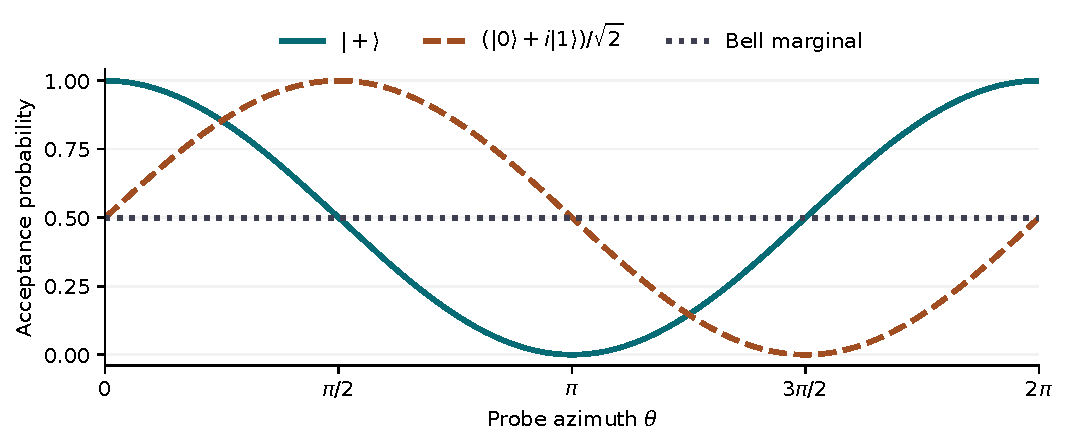
\includegraphics[width=.88\linewidth]{responses.pdf}
\caption{Born responses to an equatorial probe with azimuth $\theta$. The pure states $\ket{+}$ and $(\ket0+i\ket1)/\sqrt2$ and the reduced state of a Bell qubit all give computational probabilities $(1/2,1/2)$. Changing the probe distinguishes them. The constant line also follows by tracing out either wire of the simulated Bell state.}\label{fig:responses}
\end{figure}

A class in QAF names a collection of fields and methods. Its quantum interpretation depends on invariants and admissible operations. An amplitude class with two complex fields presents $\C^2$. Enforcing unit norm and identifying global phase gives pure qubit rays. A finite classical record type $X$ has a distinguishable encoding in the basis of $\ell^2(X)$. Deterministic classical transitions extend to channels on diagonal states. A permutation gives a unitary basis action. A many-to-one map needs an environment if implemented reversibly. A two-entry Boolean truth table has four possible classical values, so an orthogonal encoding of all tables needs two qubits. A class declaration with unrestricted arithmetic has no canonical one-qubit isomorphism.

\subsection{Five operations on functions}
Let $\mathcal A=\C^\B$. Addition, subtraction and multiplication mean pointwise arithmetic. Division $f/g$ has domain $\{(f,g):g(0)g(1)\ne0\}$ when a total two-label result is required. Composition $g\circ f$ requires the codomain of $f$ to match the domain of $g$. Two maps $\B\to\C$ therefore have no general ordinary composite. Precomposition by $h:\B\to\B$ is defined by $(f\circ h)(b)=f(h(b))$. Composition of amplitude \emph{kernels} means matrix composition $(LK)(y,x)=\sum_z L(y,z)K(z,x)$. These rules give three useful kinds of composition without coercing a complex amplitude into a wire label.

Function extensionality proves the ring laws by evaluation at each $b$. Addition and multiplication are commutative and associative, multiplication distributes over addition, and the pointwise constant functions are the respective identities. Subtraction satisfies $(f-g)+g=f$ and $f-f=0$. Wherever the quotient is defined, $(f/g)g=f$. Typed composition is associative with the corresponding identities. Neither subtraction nor division is associative in general. The Lean proofs use scalar-field laws as hypotheses. The example below executes all five operations and normalizes only at state preparation.
\inputminted[firstline=55,fontsize=\footnotesize]{qaf}{examples/prefix/algebra.qaf}
The result is $(i,1)/\sqrt2$. A zero denominator rejects evaluation. The zero function is perfectly meaningful in $\mathcal A$ and has no normalized ray. Arithmetic on representatives can also depend on phase choice: replacing $\ket0$ by $-\ket0$ leaves its ray invariant, while adding $\ket1$ then yields distinguishable rays. An operational superposition needs a phase reference and a preparation procedure. Normalizing a classical specification and evolving an unknown state by a deterministic physical channel are different interfaces. The typed preservation theorem in the archive quantifies over physical expressions whose preparations and transformations have supplied validity witnesses. It does not assert closure of all unrestricted classical expressions as pure qubits.

\section{Tensor rank, infinite width and the scope of universality}
\label{sec:infinite}
Let $H_A,H_B$ be separable complex Hilbert spaces. A unit vector in their completed Hilbert tensor product has a Schmidt expansion $\psi=\sum_{k\ge0}s_k u_k\otimes v_k$ with orthonormal families, $s_k\ge0$ and $\sum_k s_k^2=1$ \cite{schmidt,cleve}. Orthogonal projection onto the first $R$ terms leaves squared norm error $\delta_R=\sum_{k\ge R}s_k^2$. For the renormalized truncation $\psi_R$ one has $|\langle\psi,\psi_R\rangle|^2=1-\delta_R$. Its pure-state trace distance from $\psi$ is $\sqrt{\delta_R}$, which bounds the change in the probability of any effect. A specified fixed product basis also gives convergent square projections, even when it is different from the Schmidt basis. The Schmidt argument concerns a bipartition. For three or more factors a best approximation of fixed canonical tensor rank can fail to exist \cite{tensorrank}.

\textbf{Density theorem.} Choose a countable orthonormal basis of a separable $H$ and identify its coordinates with a subset of $\mathbb N^2$. For every unit vector $\psi$ and every $\epsilon>0$, there is a finite QAF \texttt{hilbert} program whose normalized state has Hilbert norm distance below $\epsilon$ after the fixed embedding. Indeed choose a finite projection whose omitted norm is below $\epsilon/4$. Approximate the retained complex coefficients by Gaussian rationals with total $\ell^2$ error below $\epsilon/4$. The resulting vector $v$ is given by a finite sum of QAF \texttt{basis} terms. The triangle inequality and $|1-\|v\||\le\|v-\psi\|$ give $\|v/\|v\|-\psi\|\le2\|v-\psi\|<\epsilon$, choosing the approximant nonzero. Finite-rank normalized density operators are similarly dense among density operators in trace norm by spectral truncation; rational pure approximants with approximated mixture weights give finite preparation ensembles. The pure-state theorem is an existence result. A procedure that selects a rank from data requires an effective tail bound.

There is an exact computational case with infinite Schmidt rank. Set
\[
 \ket{\psi_t}=\sqrt{1-t^2}\sum_{k=0}^{\infty}t^k\ket{k,k},\quad
 K(t,u)=|\langle\psi_t|\psi_u\rangle|^2
       ={(1-t^2)(1-u^2)\over(1-tu)^2}
\]
for rational $|t|,|u|<1$. The discarded mass beyond $R-1$ is $t^{2R}$. QAF also supports finite complex rational superpositions of individual basis vectors and two independently geometric product modes. Every cross term has a finite geometric-series formula for its projected inner product, and an absolutely convergent closed form at infinite rank. The evaluator computes exact rational fidelities and truncation masses. Projection can generate an ordinary QAF circuit for GPU execution. Here is a complete input.
\inputminted{qaf}{examples/prefix/hilbert.qaf}
The exact answers are $3^{-16}$, $24/25$ and $-64/225$. At rank eight the projected state's trace distance is $3^{-8}=1/6561$. This bounds the error of all effect probabilities, including ones absent from the listing. A finite cutoff alone would not give a uniform bound on expectations of an unbounded position, momentum or energy observable. Such a claim would require domain and moment estimates.

To see why the classifier has a quantum meaning, use rank-one density matrices as features in the real Hilbert space of self-adjoint Hilbert--Schmidt operators. Their inner product is $\Tr(\rho\sigma)=|\langle\psi|\phi\rangle|^2$ for pure states. This kernel is positive semidefinite since each finite Gram quadratic form is a squared Hilbert--Schmidt norm. For two training features $\rho_+$ and $\rho_-$ of unit norm and opposite labels, the minimum-norm hard-margin separator with intercept zero is $w=(\rho_+-\rho_-)/(1-\Tr(\rho_+\rho_-))$. Both constraints bind. Cauchy--Schwarz applied to their difference proves minimality. Here the training states use $t=0$ and $t=1/2$. The score at $t=1/3$ is $4(8/9-24/25)$. Its change under truncation is bounded by $\|w\|_2\sqrt{2\delta_R}$. This explicit kernel machine is an observable-derived classifier. An arbitrary learned decision score requires rescaling or calibration before interpretation as a probability.

Cortes and Vapnik's SVM optimizes a margin in a chosen feature space \cite{svm}. Chen and colleagues prove that an infinitely wide network with a suitable limiting neural tangent kernel and regularized hinge loss has the same output dynamics as a soft-margin SVM with that kernel, given matching initial outputs and the paper's smoothness and scaling conditions \cite{chen,ntk}. Their network can have nonlinear hidden layers. A predictor linear in feature coordinates can be nonlinear in its original input. A different theorem gives a hard-margin limiting direction for training certain fully connected linear networks on separable data, subject to convergence assumptions \cite{gunasekar}. The two-support classifier above uses the specified quantum fidelity kernel. Equating it to the tangent kernel of any particular deep architecture would require a derivation for that architecture.

Universal approximation likewise needs a function class and error norm. Cybenko proves uniform density on a compact cube for a family with nonlinear sigmoidal activation \cite{cybenko}. Linear layers alone compose to an affine map on their input. A linear model with an infinite feature map can nevertheless have a rich function class. A nonlinear classical representation of amplitudes is consistent with the linear evolution of the physical ket. The QAF density theorem gives a direct universality statement in the norm relevant to a quantum state, including square-integrable states lacking continuous representatives.

The quantifiers determine how far the result extends. Every separable pure state has approximants at every positive tolerance. Exact execution by a finite program has a short obstruction even for one qubit: take $\sqrt{1-p}\ket0+\sqrt p\ket1$ for $p\in[0,1]$. Measuring $\ket1\bra1$ recovers $p$ as the exact probability. There are uncountably many choices and countably many finite program texts over the language's alphabet. Supplying an arbitrary real-valued oracle as an extra input changes that statement and specifies where the missing information resides. Complete mathematical representation relative to an abstract amplitude function, approximation by executable preparations, and exact computation of particular observables therefore have different proofs.

\subsection{An executable nonlinear infinite-width network}
We can realize the nonlinear connection explicitly. Start with unit inputs $x=\rho_\psi$ in the real Hilbert--Schmidt feature space above, so $c=\langle x,y\rangle=\Tr(\rho_\psi\rho_\phi)$. Consider the scalar network $m^{-1/2}\sum_{r=1}^{m}a_r\sin(g_r(x))$, with independent standard Gaussian output weights and independent centered isonormal Gaussian families $g_r$. On every finite set of inputs their covariance matrix is the input Gram matrix. This definition avoids treating white noise as a square-summable parameter vector. Finite projections give the same construction for ordinary parameter gradients, followed by the Hilbert limit on a fixed set of inputs.

Training both weight layers in the tangent parameterization contributes one sine-product term and one cosine-product term. For jointly standard Gaussian $U,V$ of covariance $c$, the population tangent kernel is
\begin{align}
 \kappa(c)
 &=\mathbb E[\sin U\sin V]+c\,\mathbb E[\cos U\cos V] \nonumber\\
 &=e^{-1}\bigl(\sinh c+c\cosh c\bigr). \label{eq:sine}
\end{align}
The Gaussian identity $\mathbb E\cos(U\pm V)=e^{-(1\pm c)}$ proves the formula. Independent units give this deterministic kernel in the width limit by the law of large numbers on any fixed finite set of inputs. It is nonlinear in $c$ and has $\kappa(1)=1$. The limiting tangent features distinguish the classifier below from the preceding SVM using the untransformed fidelity.

For two opposite labels with unit kernel diagonal, the soft-margin dual reduces by symmetry to maximizing $2\alpha-\alpha^2[1-\kappa(c_{+-})]$ over $0\le\alpha\le C$. Taking the symmetric intercept zero gives score $\alpha[\kappa(c_{x+})-\kappa(c_{x-})]$. QAF computes both a symbolic expression and its decimal evaluation. The runnable example uses the same infinite-rank test state as before.
\inputminted{qaf}{../../examples/prefix/nonlinear.qaf}
Here $\alpha=\min\{2,1/[1-\kappa(3/4)]\}$ and the score is $\alpha[\kappa(8/9)-\kappa(24/25)]$. The independent check integrates the sine and cosine products by two-dimensional Gaussian quadrature. The result implements the infinite-width kernel classifier analytically, without fitting a large finite network. Chen et al.\ supply the training-dynamics correspondence under the assumptions stated above. The Gaussian derivation supplies the actual nonlinear kernel for this choice of features and architecture. Neither calculation increases the number of independently distinguishable states of a single quantum wire.

\section{A language whose runtime functions are qubits}
The underlying operation is a one-selector quantum multiplexor in the sense of Shende, Bullock and Markov \cite{shende}. QAF exposes its selector as a named wire that a program can invoke and later probe.
QAF has an explicit separation between a program that describes an experiment and the quantum systems in that experiment. The \texttt{fn} binding associates a function name with a qubit wire and a statically specified pair of unitary targets $U_0,U_1$. An unnamed wire can also be invoked with the default pair $(I,X)$. The operational action is
\[
 V=\ket0\bra0\otimes U_0+\ket1\bra1\otimes U_1 .
\]
Since $V^\dagger V=I$, this is a valid transformation on a superposed, mixed or entangled control. The implementation acts on the joint register. Naming a wire twice creates aliases of the same system. Using it as both selector and target in one invocation fails the distinct-wires check. The two operation descriptions belong to the invocation interface. They are classical code and additional information beyond the physical qubit. Relative phase matters: replacing $U_1$ by $-U_1$ changes the coherent control even though the isolated target gates give the same channel. The no-programming theorem requires orthogonal program states for distinguishable exact unitary channels in a deterministic universal processor \cite{noprogram}. Two program labels can select two supplied alternatives; an arbitrary unknown unitary cannot be retrieved from the amplitudes of a single qubit.

The working grammar is reproduced in Appendix~\ref{sec:grammar}. TatSu compiles the grammar to a parsing-expression-grammar parser \cite{tatsu}. The language follows the design guidance of the Zen of Python \cite{zen} through visible distinctions between state preparation, physical application, measurement, classical circuit construction and simulation-only inspection. Numerical expressions, class methods, recursion, mutable local bindings and finite loops describe amplitudes, gate entries or circuits. A \texttt{def} is a classical routine and a \texttt{proc} builds an instruction sequence. The runtime quantum-function type is the wire type. Extending the identification to every classical routine, including a routine that returns an arbitrary integer or fails to terminate, would change the meaning of either programming functions or qubits.

\inputminted[fontsize=\footnotesize]{qaf}{../../examples/prefix/recursion.qaf}
The recursive \texttt{sign} method runs for each requested basis label in the initial-state kernel. The \texttt{fan} procedure expands at compile time, yielding a Hadamard and two CNOTs in total with the explicit Hadamard in the main program. The final distribution is supported on $000$ and $111$ with probability $1/2$ each. A depth and step guard admit bounded executions and report exhaustion. In particular, a divergent recursive function is a meaningful program whose evaluation fails; it cannot denote an additional physical qubit. The grammar also supports unitary kernels, Kraus families, sequential and tensor composition, unitary adjoints, coherent selection, and before/after wrappers for slots.

\inputminted{qaf}{../../examples/prefix/functions.qaf}
The three definitions above implement three distinct constructions. The diagonal gate applies the spectral function $\exp(-i\pi Z/3)$. The two Kraus operators dephase in the $Z$ basis. The wrapper conjugates the channel with Hadamards, producing dephasing in the $X$ basis. The initial $\ket+$ is fixed by that channel, and the final Hadamard gives computational zero with probability $\cos^2(\pi/3)=1/4$. This program exercises a scalar function of an operator, a channel acting on a state and a higher-order transformation acting on a channel.

\subsection{Native execution and its reference semantics}
For a target list $w=(w_0,\ldots,w_{k-1})$ let $b[w\leftarrow x]$ replace its bits in the given order, with wire zero the leftmost displayed bit. A gate kernel produces
\[
 f'(b)=\sum_{x\in\B^k}U_{b_w,x}\,f\bigl(b[w\leftarrow x]\bigr).
\]
This is equation~\eqref{eq:isometry} applied to the usual tensor embedding of the gate. A CUDA thread computes one output amplitude, using local wire masks and its selected small matrix. The new state uses separate device storage so simultaneous updates cannot read partially written amplitudes. Scalar class fields and arithmetic in state and operation definitions are emitted to CUDA device functions. NVRTC compiles those definitions through CuPy, including supported loops and recursion \cite{cupy}. Parsing, staging, allocations and kernel launches run on the host. Query outputs cross the device boundary when requested.

An instrument introduces joint classical--quantum sectors $\rho_c$ with $\sum_c\Tr\rho_c=1$. Applying Kraus operators performs $\rho_c\mapsto\sum_a K_a\rho_c K_a^\dagger$. Measuring wire $q$ and overwriting bit $j$ maps all incoming sectors to the corresponding outgoing labels through the two projectors $P_b^{(q)}$. When different old labels lead to the same new one their masses add. A conditional selects input sectors at entry, executes its body on the selected part, and recombines it with the untouched part. This remains valid when the body overwrites its own condition bit. The CPU reference instead tracks normalized branch wavefunctions with weights. Expanding each sector as $\rho_c=\sum_{i:c_i=c}p_i\ket{\psi_i}\bra{\psi_i}$ proves by induction on instructions that the two ideal rules agree. On a physical device a single invocation samples an outcome. Exact branch probabilities are a simulator service.

For $n$ quantum wires, $m$ classical bits and local width $k$, pure-state storage per complex double buffer is $16\,2^n$ bytes, with $O(2^{n+k})$ work per dense gate. The general sector representation uses $16\,2^m4^n$ bytes per buffer. Applying $r$ dense Kraus operators uses $O(2^m4^n r4^k)$ scalar work with the direct kernel. Gate generation, query materialization and temporary buffers can raise peak memory. An NVIDIA RTX A5000 Laptop GPU executed both paths. The portable CPU path shares the same mathematical convention. Norm and Gram tests use absolute tolerance $10^{-10}$. Double precision and checks at a tolerance implement numerical predictions, with no general proof of correctly rounded evaluation for every program.

\subsection{A lossless Lean embedding}
The translator obtains a concrete TatSu derivation with labeled productions, terminals and source trivia. A Lean \texttt{Source} tree represents that derivation. A separate inductive \texttt{Term} gives a programmable embedding that users can build with Lean definitions before evaluation. The maps exchange the respective token, end, argument and rule constructors. The central proofs are short enough to reproduce directly from the checked file \cite{lean}.
\inputminted[firstline=34,lastline=38,fontsize=\footnotesize]{lean4}{../../src/qaf/lean/QAF.lean}
Structural induction proves both inverse identities on all values of the respective inductives. A spelling witness lifts the first identity to original UTF-8 source text. Preservation of any meaning assigned to the source tree follows by substitution along equality. The command-line importer evaluates the closed Lean program, decodes it and reparses its spelling to enforce membership in the canonical image of the grammar. The exporter reads back the generated Lean program and compares its tree. Edits, comments, blank lines and line endings thus have a defined round-trip path for accepted inputs. The theorem covers the embedded \texttt{Term} language. Arbitrary Lean libraries with effects or unrelated types have no implied QAF translation. The handwritten interpreter, host parser and CUDA code generator remain outside the kernel-checked proof.

\subsection{Portable execution and backend validation}
QAF's portable circuit subset starts from zeros and includes $H,X,Y,Z,S,T$, CNOT, exact Clifford decompositions of CZ and SWAP, sequences, and selected coherent or classical controls with registered rules. It accepts marginal computational probabilities and classical records. Measurement can be deferred coherently using fresh record and history wires. To overwrite a classical record, move the old value to a fresh history label and compute the new outcome into the cleared label. For nested conditions capture the branch decision in a fresh flag at entry. Orthogonal history states kill cross terms on marginalization. Induction gives the same requested statistics as immediate measurement. This is an isometric dilation and equality of the observable program semantics. The added ancillas, erased source comments and many equivalent gate schedules prevent a general source-text isomorphism to a provider program.

The Quil emitter has a separate reader. Certification checks each logical wire's ordered gate history and the terminal readout map. Identical histories permit reordering independent disjoint gates. In a common total order, slide a first instruction past disjoint instructions until it aligns with its counterpart; induction on the remaining word proves the ideal unitaries equal. Reversing CNOT's wires or swapping classical destinations is caught. Amazon Braket and Cirq adapters inspect their SDK circuit objects, while the IonQ path inspects its intermediate representation. For a compatible Google device an exact interaction-graph embedding can replace CNOT with $H$--CZ--$H$ and validate the circuit against the device. QPU calibration, compiler optimization after handoff and sampling noise are separate questions \cite{braket,cirq,azure}. Exact support for an arbitrary provider instruction must be established before admitting it.

The annealing profile describes binary or spin variables by $E(x)=c+\sum_i h_i x_i+\sum_{i<j}J_{ij}x_ix_j$. The local simulator can enumerate energies on CUDA or CPU. The D-Wave Ocean adapter reads back the binary quadratic model, including offset and variable convention, before sampling \cite{dwave}. Repeated coefficients are combined; a self-pair becomes a linear term for binary variables or a constant for spins. The one-hot example uses $(x_0+x_1+x_2-1)^2$ and has precisely three minimizers of energy zero. Arbitrary gate circuits have no transparent compilation to that annealing profile. A physical embedding and finite anneal need not find a true minimum on each read.

\begin{table}[ht]
\centering\small
\begin{tabularx}{\linewidth}{@{}lXX@{}}
\toprule Platform & Artifact exercised & Extent of evidence\\\midrule
NVIDIA CUDA & Native wavefunction, mixed-register and classical-sector kernels & Local device execution on an RTX A5000 Laptop GPU\\
CPU & Branch reference and exact rational series & Deterministic local execution\\
Amazon Braket & SDK circuit and local simulator & Circuit readback and sampled Bell support\\
Google Cirq & SDK circuit and local simulator & Circuit readback and sampled Bell support\\
Azure Quantum & Quil on hosted Rigetti QVM & 100 shots, 49 of 00 and 51 of 11\\
Azure IonQ & JSON gate payload & Offline construction and readback\\
D-Wave Ocean & Binary quadratic models & Local exact sampler and coefficient comparison\\
\bottomrule
\end{tabularx}
\caption{Execution evidence. The Azure QVM was the remotely executed target. A physical-QPU run would add evidence about a particular device and calibration.}\label{tab:platforms}
\end{table}

\subsection{Experiments and independently checkable predictions}
The following Python program checks populations, local mixing and joint coherence using the reference evaluator. The last assertion distinguishes a pure Bell state from a classical source that emits $00$ or $11$ with equal probability.
\inputminted[fontsize=\footnotesize]{python}{../../examples/check_callable.py}
For a stronger Bell test, reverse the entangler on the output or measure a joint $X\otimes X$ observable. A Bell state gives expectation one while the equally weighted incoherent mixture of $00$ and $11$ gives zero. The hosted 100-shot Bell run measured in the computational basis, so it checked readout correspondence and the expected support without measuring entanglement. No physical QPU benchmark or speedup estimate follows from these counts.

Other deterministic checks exercise teleportation of a state with a complex relative phase in all four outcome branches, Grover search, order finding, the Toffoli decomposition on all eight input columns including phases, and seeded arbitrary-input gates on permuted wires. Reconstruction tests compare Bloch, SIC, Wigner and Choi forms. A process example checks memory under two interventions. The singular-value example compares the dilated circuit block with its closed polynomial. For the Dirichlet box $(0,1)$ in units $\hbar=m=1$, $N=2^n$ interior points give ground energy $2(N+1)^2\sin^2(\pi/[2(N+1)])$. It converges from below to $\pi^2/2$. The associated infinite series example checks exact overlaps against normalized finite QAF preparations. All tests and numerical outputs are supplied with the paper.

\section{Factoring with the same program on two amplitude representations}
Elegance is the design objective for this experiment. The ordinary Shor program uses the same modular-power and Fourier routines as a short-discrete-logarithm factoring variant. Input consists of the public modulus, the chosen base and register sizes derived from the modulus. No prime factor or order appears in circuit construction. One native modular operation multiplies by a unit modulo $N$ on labels below $N$ and fixes the remaining labels. A fixed control selects this permutation or the identity. On a GPU, inverting the multiplier with Euclid's algorithm lets each output thread read its unique input. This uses one state-vector pass per multiplication and avoids constructing a dense matrix. A fault-tolerant device must pay for reversible modular arithmetic. The costs of the two implementations have different units.

For ordinary order finding the state before the inverse Fourier transform is proportional to $\sum_a\ket a\ket{g^a\bmod N}$. For the short-log algorithm choose an odd $N=pq$ with distinct, equal-bit-length primes, with $b$ bits per prime and $m=b-1$. Define $d=(p+q-2)/2-2^m$. This is nonnegative and below $2^m$. For a suitable $g\in\mathbb{Z}_N^*$ the known element $x=g^{(N-1)/2-2^m}\bmod N$ satisfies $x=g^d$, since the difference of the exponents is $\varphi(N)/2$, a multiple of both $p-1$ and $q-1$. The order of $g$ must distinguish the desired short logarithm. Two coherent exponents produce $g^a x^{-c}$ in the work register. Fourier transformation of both exponent registers yields a frequency pair. Classical lattice post-processing recovers a candidate $d$. The two roots of $z^2-2(d+2^m+1)z+N$ give factors, each verified by exact integer arithmetic \cite{eh,shortpost,shortsuccess}.

\inputminted[firstline=100,fontsize=\footnotesize]{qaf}{examples/prefix/factoring.qaf}
The register roles in this listing are explicit. The first exponent has $m+\ell$ wires and the second has $\ell$ wires. The work register begins at their combined width. Base-two order finding modulo 21 used fifteen wires and recovered order six, giving $3\cdot7$. The balanced short-log instance modulo 143 used seventeen wires with $m=\ell=3$. It recovered $d=3$, yielding $11\cdot13$. The first sampled pair was $(51,5)$. All sixteen seeded samples in each small experiment yielded verified factors with the selected post-processing parameters. These frequencies come from the simulated circuit. The independent reference enumerates the public modular function on its exponent registers and Fourier transforms each work-label indicator. It agrees with every marginal probability to within $6.2\times10^{-16}$ on the two examples. The reference supplies no period to the execution. Quaspy provides the classical post-processing routines \cite{orderpost,quaspy}.

As of 8 November 2026, optimizing RSA factoring depends on a physical model and a cost objective. Gidney combines approximate residue arithmetic with fault-tolerant resource choices \cite{gidney}. The Pinnacle architecture considers quantum LDPC codes, and reconfigurable-atom analyses explore different time--space tradeoffs \cite{pinnacle,oratomic}. Pappalardo and colleagues' October cat-qubit preprint gives one estimate of 22,593 physical qubits and 3.14 days for RSA-2048 under a one-microsecond error-correction cycle, ten-microsecond reaction, specified phase-flip noise and negligible bit flips \cite{catshor}. A different operating point in that work spends more qubits for a shorter schedule. These are projections. Our demonstrations implement the logical Fourier and modular computations on a classical GPU. They do not implement the resource papers' physical codes, magic-state factories, layouts or RSA-2048 schedules. The general classical simulation still scales exponentially.

\subsection{When the whole network denotes a qubit}
Let $F_\theta:\{0,1\}\to\C$ be the output of an entire network and require $0<\sum_b|F_\theta(b)|^2<\infty$. Its denotation is the ray of $F_\theta/\|F_\theta\|$. An embedding with two complex basis weights represents every such ray in the ideal parameter model. Define $\theta\sim\theta'$ when these denotations coincide. Mapping an equivalence class to its ray is injective by definition and surjective onto the reachable rays. \texttt{Networks.lean} proves this fact for any preparation map. For this architecture its image is all pure qubits. For raw weights the preparation is many-to-one: $(1,0)$ and $(2,0)$ give the same qubit. A register with $n$ inputs initially represents a product of normalized two-label functions. As a circuit runs, the backend evaluates the resulting joint function on $\B^n$.

We executed the same seventeen-wire prefix file under native CUDA and a PyTorch amplitude backend. In PyTorch the input wire was an instance of \texttt{BasisAmplitudes} initialized with trainable weights $(2,0)$, whose normalized vector is $\ket0$. The existing first $X$ and every subsequent modular and Fourier operation were taken directly from the source. Comparing all $131{,}072$ output amplitudes gave maximum absolute difference $5.21\times10^{-18}$ or less. The check compares complex amplitudes, including relative phases, before sampling. It establishes equivalence on this run. On entangled intermediate states the representation is a joint amplitude computation.

The same language can declare a general feedforward network directly. This network supplies the real and imaginary parts of a spatial amplitude.
\inputminted{qaf}{examples/prefix/wave_net.qaf}
The exporter produces ordinary runnable PyTorch \cite{torch}. It uses the same declared layer ordering as the live \texttt{nn.Sequential} model. The example loads identical parameters in the generated and live modules and compares their outputs.
\inputminted[fontsize=\footnotesize]{python}{examples/wave_net.py}
For the box problem set $\psi_j\propto x_j(1-x_j)(u_\theta(x_j)+i v_\theta(x_j))$ on 40 interior nodes. The optimizer differentiates the Rayleigh quotient of the actual tridiagonal Dirichlet Hamiltonian on the GPU. It reduced the energy from $5.48168220$ to $4.93238870$. The independent grid eigenvalue is $4.93238821$, while the continuum ground energy is $4.93480220$. The first discrepancy measures variational error at the selected grid size, and the second comparison includes spatial discretization. A uniform approximation theorem for continuous functions would not by itself certify either error. Energy convergence for an unbounded Hamiltonian requires control in its form domain.

\subsection{One build, two representations}
\texttt{build\_qaf.py} takes one circuit file and creates an executable CUDA plan together with a Lean \texttt{Program.lean}. The build also contains generated CUDA expressions, the device kernels, the input state and gate tables, and a manifest with content hashes. The verify step reloads the exported plan, compiles its saved CUDA kernels and replays it without parsing QAF. It also evaluates the Lean program and checks that its recovered UTF-8 bytes equal the original. For the factoring program CUDA replay was bit-identical to direct native execution. The Lean source isomorphism is a theorem over the embedding. CUDA replay is an execution check. A separate Lean theorem identifies the portable instruction datatype with its supported Quil-line datatype in both directions. A full proof about floating-point execution, GPU drivers or a provider optimizer remains open.

\section{Conclusion}
On one wire, a basis-amplitude function and a pure qubit carry the same information once norm and phase are handled. The response to effects extends the construction to every mixed qubit. On many wires the domain grows by tensor product, and prefix splitting retains the correlations that single-wire wavefunctions would lose. In QAF a programmer can call the same wire whose responses they measure. The Bell example consequently tests the language's central design in six lines. The strongest demonstrated portability result concerns the reconstructed ideal gate word and its readout. Further work toward an end-to-end verified compiler must connect a verified parser, operational semantics, target lowering and numerical execution to the existing Lean theorems.
\appendix
\noindent The manuscript, runnable examples, compiler and proofs are available in the
\href{https://github.com/mingusb/qubit-as-a-function}{Qubit-as-a-Function repository}.
\section{Complete concrete grammar}
\label{sec:grammar}
The paper prints QAF's prefix surface. Its complete TatSu reader appears first. A parenthesized form and the same form written with indented operands have identical structure. The layout pass groups a line with its indented children and closes it at the next sibling or dedent. The first line selects the surface. Fixed-arity scalar functions can consume operands inline. The reference manual in the source describes the special forms and their expansion into the typed interpreter.
\inputminted[fontsize=\footnotesize]{qafgrammar}{../../src/qaf/prefix.ebnf}
The following TatSu grammar defines the shared expression and statement forms after lowering. A production labels fields consumed by semantic actions. Parentheses group, braces repeat and a dollar sign matches end of input. In conventional QAF source, indentation can also replace explicit braces. A colon at the end of a block header and terminal semicolons are optional. The source bridge retains original spelling, comments and layout.
\inputminted[fontsize=\footnotesize]{qafgrammar}{../../src/qaf/qaf.ebnf}
\section{Reproducing the artifact}
The companion distribution contains the grammar, CLI, Python interpreter, CUDA kernels, provider adapters, Lean files, worked programs, numerical checks, bibliography and manuscript source. The README gives the tested versions and build commands. Generated examples and figures can be recreated locally. The saved hosted-job receipt records its target, status, shots, outcome counts and gate certificate. Rebuilding the paper requires the supplied \texttt{qaf} and \texttt{qafgrammar} Pygments lexers when refreshing the minted cache. Listings include the real source files used by the examples and proof checker. The \texttt{quantumarticle} class is used for typesetting.
\begin{thebibliography}{999}
\bibitem{planck} M. Planck. \href{https://doi.org/10.1002/andp.19013090310}{Ueber das Gesetz der Energieverteilung im Normalspectrum}. \emph{Annalen der Physik} 309 553-563 (1901).
\bibitem{einstein} A. Einstein. \href{https://doi.org/10.1002/andp.19053220607}{Über einen die Erzeugung und Verwandlung des Lichtes betreffenden heuristischen Gesichtspunkt}. \emph{Annalen der Physik} 322 132-148 (1905).
\bibitem{heisenberg} W. Heisenberg. \href{https://doi.org/10.1007/BF01328377}{Über quantentheoretische Umdeutung kinematischer und mechanischer Beziehungen}. \emph{Zeitschrift für Physik} 33 879-893 (1925).
\bibitem{schrodinger} E. Schrödinger. \href{https://doi.org/10.1103/PhysRev.28.1049}{An Undulatory Theory of the Mechanics of Atoms and Molecules}. \emph{Physical Review} 28 1049-1070 (1926).
\bibitem{born} M. Born. \href{https://doi.org/10.1007/BF01397477}{Zur Quantenmechanik der Stossvorgänge}. \emph{Zeitschrift für Physik} 37 863-867 (1926).
\bibitem{dirac} P. A. M. Dirac. \href{https://doi.org/10.1098/rspa.1927.0012}{The physical interpretation of the quantum dynamics}. \emph{Proceedings of the Royal Society of London. Series A, Containing Papers of a Mathematical and Physical Character} 113 621-641 (1927).
\bibitem{gleason} A. Gleason. \href{https://doi.org/10.1512/iumj.1957.6.56050}{Measures on the Closed Subspaces of a Hilbert Space}. \emph{Indiana University Mathematics Journal} 6 885-893 (1957).
\bibitem{busch} P. Busch. \href{https://doi.org/10.1103/PhysRevLett.91.120403}{Quantum States and Generalized Observables: A Simple Proof of Gleason's Theorem}. \emph{Physical Review Letters} 91 120403 (2003).
\bibitem{qubitgleason} V. Fiorentino, S. Weigert. \href{https://arxiv.org/abs/2511.15607}{Gleason's Theorem for a Qubit as Part of a Composite System}. \emph{arXiv:2511.15607}  (2025).
\bibitem{epr} A. Einstein, B. Podolsky, N. Rosen. \href{https://doi.org/10.1103/PhysRev.47.777}{Can Quantum-Mechanical Description of Physical Reality Be Considered Complete?}. \emph{Physical Review} 47 777-780 (1935).
\bibitem{bell} J. S. Bell. \href{https://doi.org/10.1103/PhysicsPhysiqueFizika.1.195}{On the Einstein Podolsky Rosen paradox}. \emph{Physics Physique Fizika} 1 195-200 (1964).
\bibitem{chsh} J. F. Clauser, M. A. Horne, A. Shimony, R. A. Holt. \href{https://doi.org/10.1103/PhysRevLett.23.880}{Proposed Experiment to Test Local Hidden-Variable Theories}. \emph{Physical Review Letters} 23 880-884 (1969).
\bibitem{ks} S. Kochen, E. Specker. \href{https://doi.org/10.1512/iumj.1968.17.17004}{The Problem of Hidden Variables in Quantum Mechanics}. \emph{Indiana University Mathematics Journal} 17 59-87 (1967).
\bibitem{spekkens} R. W. Spekkens. \href{https://doi.org/10.1103/PhysRevA.71.052108}{Contextuality for preparations, transformations, and unsharp measurements}. \emph{Physical Review A} 71 052108 (2005).
\bibitem{ptm} D. Schmid, R. D. Baldijão, J. H. Selby, A. B. Sainz, R. W. Spekkens. \href{https://doi.org/10.22331/q-2026-10-27-2250}{Noncontextuality inequalities for prepare-transform-measure scenarios}. \emph{Quantum} 10 2250 (2026).
\bibitem{wigner} E. Wigner. \href{https://doi.org/10.1103/PhysRev.40.749}{On the Quantum Correction For Thermodynamic Equilibrium}. \emph{Physical Review} 40 749-759 (1932).
\bibitem{husimi} K. Husimi. \href{https://www.jstage.jst.go.jp/article/ppmsj1919/22/4/22_4_264/_article}{Some Formal Properties of the Density Matrix}. \emph{Proc. Phys.-Math. Soc. Japan 22, 264--314}  (1940).
\bibitem{glauber} R. J. Glauber. \href{https://doi.org/10.1103/PhysRev.131.2766}{Coherent and Incoherent States of the Radiation Field}. \emph{Physical Review} 131 2766-2788 (1963).
\bibitem{sudarshan} E. C. G. Sudarshan. \href{https://doi.org/10.1103/PhysRevLett.10.277}{Equivalence of Semiclassical and Quantum Mechanical Descriptions of Statistical Light Beams}. \emph{Physical Review Letters} 10 277-279 (1963).
\bibitem{wootters} W. K. Wootters. \href{https://doi.org/10.1016/0003-4916(87)90176-X}{A Wigner-function formulation of finite-state quantum mechanics}. \emph{Annals of Physics} 176 1-21 (1987).
\bibitem{frame} C. Ferrie, J. Emerson. \href{https://doi.org/10.1088/1751-8113/41/35/352001}{Frame representations of quantum mechanics and the necessity of negativity in quasi-probability representations}. \emph{Journal of Physics A: Mathematical and Theoretical} 41 352001 (2008).
\bibitem{kd} D. Schmid, R. D. Baldijão, Y. Yīng, R. Wagner, J. H. Selby. \href{https://doi.org/10.1103/PhysRevA.110.052206}{Kirkwood-Dirac representations beyond quantum states and their relation to noncontextuality}. \emph{Physical Review A} 110 052206 (2024).
\bibitem{sic} J. M. Renes, R. Blume-Kohout, A. J. Scott, C. M. Caves. \href{https://doi.org/10.1063/1.1737053}{Symmetric informationally complete quantum measurements}. \emph{Journal of Mathematical Physics} 45 2171-2180 (2004).
\bibitem{bargmann} V. Bargmann. \href{https://doi.org/10.1002/cpa.3160140303}{On a Hilbert space of analytic functions and an associated integral transform part I}. \emph{Communications on Pure and Applied Mathematics} 14 187-214 (1961).
\bibitem{majorana} E. Majorana. \href{https://doi.org/10.1007/BF02960953}{Atomi orientati in campo magnetico variabile}. \emph{Il Nuovo Cimento} 9 43-50 (1932).
\bibitem{holocode} M. W. AlMasri. \href{https://arxiv.org/abs/2609.19162}{Holomorphic Quantum Error Correction Codes}. \emph{arXiv:2609.19162}  (2026).
\bibitem{field} O. Éboli, R. Jackiw, S. Pi. \href{https://doi.org/10.1103/PhysRevD.37.3557}{Quantum fields out of thermal equilibrium}. \emph{Physical Review D} 37 3557-3581 (1988).
\bibitem{feynman} R. P. Feynman. \href{https://doi.org/10.1007/BF02650179}{Simulating physics with computers}. \emph{International Journal of Theoretical Physics} 21 467-488 (1982).
\bibitem{deutsch} D. Deutsch. \href{https://doi.org/10.1098/rspa.1985.0070}{Quantum theory, the Church--Turing principle and the universal quantum computer}. \emph{Proceedings of the Royal Society of London. A. Mathematical and Physical Sciences} 400 97-117 (1985).
\bibitem{bv} E. Bernstein, U. Vazirani. \href{https://doi.org/10.1137/S0097539796300921}{Quantum Complexity Theory}. \emph{SIAM Journal on Computing} 26 1411-1473 (1997).
\bibitem{schumacher} B. Schumacher. \href{https://doi.org/10.1103/PhysRevA.51.2738}{Quantum coding}. \emph{Physical Review A} 51 2738-2747 (1995).
\bibitem{noclone} W. K. Wootters, W. H. Zurek. \href{https://doi.org/10.1038/299802a0}{A single quantum cannot be cloned}. \emph{Nature} 299 802-803 (1982).
\bibitem{dj} D. Deutsch, R. Jozsa. \href{https://doi.org/10.1098/rspa.1992.0167}{Rapid solution of problems by quantum computation}. \emph{Proceedings of the Royal Society of London. Series A: Mathematical and Physical Sciences} 439 553-558 (1992).
\bibitem{shor} P. W. Shor. \href{https://doi.org/10.1137/S0097539795293172}{Polynomial-Time Algorithms for Prime Factorization and Discrete Logarithms on a Quantum Computer}. \emph{SIAM Journal on Computing} 26 1484-1509 (1997).
\bibitem{grover} L. K. Grover. \href{https://doi.org/10.1145/237814.237866}{A fast quantum mechanical algorithm for database search}. \emph{Proceedings of the twenty-eighth annual ACM symposium on Theory of computing - STOC '96} 212-219 (1996).
\bibitem{barenco} A. Barenco, C. H. Bennett, R. Cleve, et al. \href{https://doi.org/10.1103/PhysRevA.52.3457}{Elementary gates for quantum computation}. \emph{Physical Review A} 52 3457-3467 (1995).
\bibitem{boykin} P. O. Boykin, T. Mor, M. Pulver, V. Roychowdhury, F. Vatan. \href{https://doi.org/10.1109/SFFCS.1999.814621}{On universal and fault-tolerant quantum computing: a novel basis and a new constructive proof of universality for Shor's basis}. \emph{40th Annual Symposium on Foundations of Computer Science (Cat. No.99CB37039)} 486-494 (1999).
\bibitem{sk} C. M. Dawson, M. A. Nielsen. \href{https://arxiv.org/abs/quant-ph/0505030}{The Solovay-Kitaev algorithm}. \emph{arXiv:quant-ph/0505030}  (2005).
\bibitem{error} P. W. Shor. \href{https://doi.org/10.1103/PhysRevA.52.R2493}{Scheme for reducing decoherence in quantum computer memory}. \emph{Physical Review A} 52 R2493-R2496 (1995).
\bibitem{teleport} C. H. Bennett, G. Brassard, C. Crépeau, et al. \href{https://doi.org/10.1103/PhysRevLett.70.1895}{Teleporting an unknown quantum state via dual classical and Einstein-Podolsky-Rosen channels}. \emph{Physical Review Letters} 70 1895-1899 (1993).
\bibitem{threshold} Google Quantum AI and Collaborators, R. Acharya, D. A. Abanin, et al. \href{https://doi.org/10.1038/s41586-024-08449-y}{Quantum error correction below the surface code threshold}. \emph{Nature} 638 920-926 (2024).
\bibitem{universalqc} H. Zhou, C. Zhao, M. Cain, et al. \href{https://doi.org/10.1038/s41586-025-09543-5}{Low-overhead transversal fault tolerance for universal quantum computation}. \emph{Nature} 646 303-308 (2025).
\bibitem{category} S. Abramsky, B. Coecke. \href{https://arxiv.org/abs/quant-ph/0402130}{A categorical semantics of quantum protocols}. \emph{arXiv:quant-ph/0402130}  (2004).
\bibitem{jam} A. Jamiolkowski. \href{https://doi.org/10.1016/0034-4877(72)90011-0}{Linear transformations which preserve trace and positive semidefiniteness of operators}. \emph{Reports on Mathematical Physics} 3 275-278 (1972).
\bibitem{choi} M. Choi. \href{https://doi.org/10.1016/0024-3795(75)90075-0}{Completely positive linear maps on complex matrices}. \emph{Linear Algebra and its Applications} 10 285-290 (1975).
\bibitem{stine} W. F. Stinespring. \href{https://doi.org/10.2307/2032342}{Positive Functions on C * -Algebras}. \emph{Proceedings of the American Mathematical Society} 6 211 (1955).
\bibitem{zx} B. Coecke, R. Duncan. \href{https://arxiv.org/abs/0906.4725}{Interacting Quantum Observables: Categorical Algebra and Diagrammatics}. \emph{arXiv:0906.4725}  (2009).
\bibitem{qset} A. Kornell. \href{https://arxiv.org/abs/1804.00581}{Quantum sets}. \emph{arXiv:1804.00581}  (2018).
\bibitem{effectus} K. Cho, B. Jacobs, B. Westerbaan, A. Westerbaan. \href{https://arxiv.org/abs/1512.05813}{An Introduction to Effectus Theory}. \emph{arXiv:1512.05813}  (2015).
\bibitem{qpl} P. Selinger. \href{https://doi.org/10.1017/S0960129504004256}{Towards a quantum programming language}. \emph{Mathematical Structures in Computer Science} 14 527-586 (2004).
\bibitem{lambda} P. Selinger, B. Valiron. \href{https://arxiv.org/abs/cs/0404056}{A lambda calculus for quantum computation with classical control}. \emph{arXiv:cs/0404056}  (2004).
\bibitem{qml} T. Altenkirch, J. Grattage. \href{https://arxiv.org/abs/quant-ph/0409065}{A functional quantum programming language}. \emph{arXiv:quant-ph/0409065}  (2004).
\bibitem{arrows} J. K. Vizzotto, T. Altenkirch, A. Sabry. \href{https://arxiv.org/abs/quant-ph/0501151}{Structuring quantum effects: superoperators as arrows}. \emph{arXiv:quant-ph/0501151}  (2005).
\bibitem{quipper} A. S. Green, P. L. Lumsdaine, N. J. Ross, P. Selinger, B. Valiron. \href{https://arxiv.org/abs/1304.3390}{Quipper: A Scalable Quantum Programming Language}. \emph{arXiv:1304.3390}  (2013).
\bibitem{proto} F. Rios, P. Selinger. \href{https://arxiv.org/abs/1706.02630}{A Categorical Model for a Quantum Circuit Description Language (Extended Abstract)}. \emph{arXiv:1706.02630}  (2017).
\bibitem{qwire} J. Paykin, R. Rand, S. Zdancewic. \href{https://doi.org/10.1145/3009837.3009894}{QWIRE: a core language for quantum circuits}. \emph{Proceedings of the 44th ACM SIGPLAN Symposium on Principles of Programming Languages} 846-858 (2017).
\bibitem{silq} B. Bichsel, M. Baader, T. Gehr, M. Vechev. \href{https://doi.org/10.1145/3385412.3386007}{Silq: a high-level quantum language with safe uncomputation and intuitive semantics}. \emph{Proceedings of the 41st ACM SIGPLAN Conference on Programming Language Design and Implementation} 286-300 (2020).
\bibitem{qunity} F. Voichick, L. Li, R. Rand, M. Hicks. \href{https://arxiv.org/abs/2204.12384}{Qunity: A Unified Language for Quantum and Classical Computing (Extended Version)}. \emph{arXiv:2204.12384}  (2022).
\bibitem{lambdapc} J. Paykin, S. Winnick. \href{https://arxiv.org/abs/2407.16801}{Qudit Quantum Programming with Projective Cliffords}. \emph{arXiv:2407.16801}  (2024).
\bibitem{cpos} A. Kornell, B. Lindenhovius, M. Mislove. \href{https://doi.org/10.1017/S096012952610053X}{Categories of quantum cpos}. \emph{Mathematical Structures in Computer Science} 36 e15 (2026).
\bibitem{super} G. Chiribella, G. M. D'Ariano, P. Perinotti. \href{https://doi.org/10.1209/0295-5075/83/30004}{Transforming quantum operations: Quantum supermaps}. \emph{EPL (Europhysics Letters)} 83 30004 (2008).
\bibitem{combs} G. Chiribella, G. M. D'Ariano, P. Perinotti. \href{https://doi.org/10.1103/PhysRevA.80.022339}{Theoretical framework for quantum networks}. \emph{Physical Review A} 80 022339 (2009).
\bibitem{process} F. A. Pollock, C. Rodríguez-Rosario, T. Frauenheim, M. Paternostro, K. Modi. \href{https://doi.org/10.1103/PhysRevLett.120.040405}{Operational Markov Condition for Quantum Processes}. \emph{Physical Review Letters} 120 040405 (2018).
\bibitem{switch} G. Chiribella, G. M. D'Ariano, P. Perinotti, B. Valiron. \href{https://doi.org/10.1103/PhysRevA.88.022318}{Quantum computations without definite causal structure}. \emph{Physical Review A} 88 022318 (2013).
\bibitem{indef} O. Oreshkov, F. Costa, Č. Brukner. \href{https://doi.org/10.1038/ncomms2076}{Quantum correlations with no causal order}. \emph{Nature Communications} 3 1092 (2012).
\bibitem{projectors} T. Hoffreumon, O. Oreshkov. \href{https://doi.org/10.22331/q-2026-01-21-1978}{Projective characterization of higher-order quantum transformations}. \emph{Quantum} 10 1978 (2026).
\bibitem{jencova} A. Jenčová. \href{https://doi.org/10.22331/q-2026-05-05-2090}{On the structure of higher order quantum maps}. \emph{Quantum} 10 2090 (2026).
\bibitem{jpos} A. Jenčová. \href{https://arxiv.org/abs/2604.09192}{Order structure and signalling in higher order quantum maps}. \emph{arXiv:2604.09192}  (2026).
\bibitem{causaldecomp} T. van der Lugt, R. Lorenz. \href{https://doi.org/10.22331/q-2026-09-30-2218}{Unitary causal decompositions: a characterisation via lattice theory}. \emph{Quantum} 10 2218 (2026).
\bibitem{guide} P. Taranto, S. Milz, M. Murao, M. T. Quintino, K. Modi. \href{https://doi.org/10.1103/92c4-g7qs}{A Guide to Higher-order quantum operations}. \emph{PRX Quantum, accepted June 9}  (2026).
\bibitem{granthi} S. Abramsky, R. Jagadeesan. \href{https://arxiv.org/abs/2608.20443}{Granthi: Higher-Order Quantum Programming via Unitary Wiring}. \emph{arXiv:2608.20443}  (2026).
\bibitem{causaltype} K. Barsse, R. Péchoux, S. Perdrix. \href{https://arxiv.org/abs/2607.09534}{Higher-Order Programs with Indefinite Causal Orders: a Linear Approach to Coherent Control of Quantum Processes}. \emph{arXiv:2607.09534}  (2026).
\bibitem{purecontrol} K. Hirata, T. Tsukada. \href{https://arxiv.org/abs/2607.15926}{Causality in Pure Quantum Computation with Quantum Control}. \emph{arXiv:2607.15926}  (2026).
\bibitem{closedlabs} M. Salzger, V. Vilasini. \href{https://arxiv.org/abs/2605.08351}{Higher-order quantum processes respecting closed labs in a spacetime have quantum controlled causal order}. \emph{arXiv:2605.08351}  (2026).
\bibitem{essential} S. Abramsky, R. Jagadeesan. \href{https://arxiv.org/abs/2606.04080}{Essential Unitarity for Higher-Order Quantum Computation}. \emph{arXiv:2606.04080}  (2026).
\bibitem{quasip} N. D. Ahmed, R. Kunjwal. \href{https://arxiv.org/abs/2610.00579}{Characterizing unitaries via quasi-process functions}. \emph{arXiv:2610.00579}  (2026).
\bibitem{loglambda} K. Tokuo. \href{https://arxiv.org/abs/2610.34266}{A Lambda Calculus Based on Quantum Logic}. \emph{arXiv:2610.34266}  (2026).
\bibitem{indirect} S. Vedl, V. Srivastava, R. Ghosh, A. Gilchrist. \href{https://arxiv.org/abs/2609.18409}{Benchmarking indirect quantum control schemes via higher-order quantum operations}. \emph{arXiv:2609.18409}  (2026).
\bibitem{qsp} G. H. Low, I. L. Chuang. \href{https://doi.org/10.1103/PhysRevLett.118.010501}{Optimal Hamiltonian Simulation by Quantum Signal Processing}. \emph{Physical Review Letters} 118 010501 (2017).
\bibitem{qubitization} G. H. Low, I. L. Chuang. \href{https://doi.org/10.22331/q-2019-07-12-163}{Hamiltonian Simulation by Qubitization}. \emph{Quantum} 3 163 (2019).
\bibitem{qsvt} A. Gilyén, Y. Su, G. H. Low, N. Wiebe. \href{https://doi.org/10.1145/3313276.3316366}{Quantum singular value transformation and beyond: exponential improvements for quantum matrix arithmetics}. \emph{Proceedings of the 51st Annual ACM SIGACT Symposium on Theory of Computing} 193-204 (2019).
\bibitem{grand} J. M. Martyn, Z. M. Rossi, A. K. Tan, I. L. Chuang. \href{https://doi.org/10.1103/PRXQuantum.2.040203}{Grand Unification of Quantum Algorithms}. \emph{PRX Quantum} 2 040203 (2021).
\bibitem{qn} X. Lu, Y. Liu, H. Lin. \href{https://doi.org/10.22331/q-2026-03-27-2048}{Quantum Signal Processing and Quantum Singular Value Transformation on U(N)}. \emph{Quantum} 10 2048 (2026).
\bibitem{mqsp} G. H. Low. \href{https://arxiv.org/abs/2610.01125}{Multivariate Quantum Signal Processing}. \emph{arXiv:2610.01125}  (2026).
\bibitem{linearqsp} M. Arsenault, H. Kristjánsson. \href{https://arxiv.org/abs/2608.14387}{Linearised quantum signal processing}. \emph{arXiv:2608.14387}  (2026).
\bibitem{arbmatrix} X. Gutiérrez, L. Laneve, M. Sanz. \href{https://arxiv.org/abs/2604.19688}{Quantum Eigenvalue Transformations for Arbitrary Matrices}. \emph{arXiv:2604.19688}  (2026).
\bibitem{recentqsp} T. Gurfinkel, K. De Silva, A. Mahasinghe, et al. \href{https://arxiv.org/abs/2609.09977}{From Block-encoding to Generalized Quantum Signal Processing: Principles, Algorithms and Applications}. \emph{arXiv:2609.09977}  (2026).
\bibitem{trotter26} G. Rendón. \href{https://doi.org/10.22331/q-2026-11-06-2261}{All you need is Trotter}. \emph{Quantum} 10 2261 (2026).
\bibitem{schmidt} E. Schmidt. \href{https://doi.org/10.1007/BF01449770}{Zur Theorie der linearen und nichtlinearen Integralgleichungen}. \emph{Mathematische Annalen} 63 433-476 (1907).
\bibitem{cleve} R. Cleve. \href{https://cleve.iqc.uwaterloo.ca/resources/Qic890LectureNotes2019Apr22\%28V22\%29.pdf}{Introduction to Quantum Information Processing}. \emph{University of Waterloo, QIC 890 lecture notes}  (2019).
\bibitem{tensorrank} V. de Silva, L. Lim. \href{https://doi.org/10.1137/06066518X}{Tensor Rank and the Ill-Posedness of the Best Low-Rank Approximation Problem}. \emph{SIAM Journal on Matrix Analysis and Applications} 30 1084-1127 (2008).
\bibitem{svm} C. Cortes, V. Vapnik. \href{https://doi.org/10.1007/BF00994018}{Support-vector networks}. \emph{Machine Learning} 20 273-297 (1995).
\bibitem{chen} Y. Chen, W. Huang, L. M. Nguyen, T.-W. Weng. \href{https://proceedings.neurips.cc/paper/2021/hash/c559da2ba967eb820766939a658022c8-Abstract.html}{On the Equivalence between Neural Network and Support Vector Machine}. \emph{NeurIPS 34}  (2021).
\bibitem{ntk} A. Jacot, F. Gabriel, C. Hongler. \href{https://arxiv.org/abs/1806.07572}{Neural Tangent Kernel: Convergence and Generalization in Neural Networks}. \emph{NeurIPS 31}  (2018).
\bibitem{gunasekar} S. Gunasekar, J. D. Lee, D. Soudry, N. Srebro. \href{https://proceedings.neurips.cc/paper/2018/hash/0e98aeeb54acf612b9eb4e48a269814c-Abstract.html}{Implicit Bias of Gradient Descent on Linear Convolutional Networks}. \emph{NeurIPS 31}  (2018).
\bibitem{cybenko} G. Cybenko. \href{https://doi.org/10.1007/BF02551274}{Approximation by superpositions of a sigmoidal function}. \emph{Mathematics of Control, Signals, and Systems} 2 303-314 (1989).
\bibitem{noprogram} M. A. Nielsen, I. L. Chuang. \href{https://doi.org/10.1103/PhysRevLett.79.321}{Programmable Quantum Gate Arrays}. \emph{Physical Review Letters} 79 321-324 (1997).
\bibitem{tatsu} TatSu project. \href{https://tatsu.readthedocs.io/en/stable/}{TatSu documentation}. \emph{Stable documentation, accessed November 8}  (2026).
\bibitem{zen} T. Peters. \href{https://peps.python.org/pep-0020/}{PEP 20 -- The Zen of Python}. \emph{Python Enhancement Proposals}  (2004).
\bibitem{cupy} CuPy project. \href{https://docs.cupy.dev/en/stable/user_guide/kernel.html}{CuPy user-defined kernels}. \emph{Documentation, accessed November 8}  (2026).
\bibitem{lean} Lean project. \href{https://lean-lang.org/doc/reference/latest/}{The Lean Language Reference}. \emph{Documentation, accessed November 8}  (2026).
\bibitem{braket} Amazon Web Services. \href{https://docs.aws.amazon.com/braket/latest/developerguide/what-is-braket.html}{Amazon Braket Developer Guide}. \emph{Documentation, accessed November 8}  (2026).
\bibitem{cirq} Google Quantum AI. \href{https://quantumai.google/cirq}{Cirq}. \emph{Documentation, accessed November 8}  (2026).
\bibitem{azure} Microsoft. \href{https://learn.microsoft.com/en-us/azure/quantum/provider-rigetti}{Rigetti provider}. \emph{Azure Quantum documentation, accessed November 8}  (2026).
\bibitem{dwave} D-Wave. \href{https://docs.dwavequantum.com/en/latest/ocean/}{Ocean software}. \emph{Documentation, accessed November 8}  (2026).
\bibitem{eh} M. Ekerå, J. Håstad. \href{https://arxiv.org/abs/1702.00249}{Quantum algorithms for computing short discrete logarithms and factoring RSA integers}. \emph{arXiv:1702.00249}  (2017).
\bibitem{shortpost} M. Ekerå. \href{https://doi.org/10.1007/s10623-020-00783-2}{On post-processing in the quantum algorithm for computing short discrete logarithms}. \emph{Designs, Codes and Cryptography} 88 2313-2335 (2020).
\bibitem{shortsuccess} M. Ekerå. \href{https://arxiv.org/abs/2309.01754}{On the success probability of the quantum algorithm for the short DLP}. \emph{arXiv:2309.01754}  (2023).
\bibitem{orderpost} M. Ekerå. \href{https://doi.org/10.1145/3655026}{On the Success Probability of Quantum Order Finding}. \emph{ACM Transactions on Quantum Computing} 5 1-40 (2024).
\bibitem{quaspy} M. Ekerå. \href{https://github.com/ekera/quaspy}{Quaspy: quantum algorithm simulation in Python}. \emph{Reference implementation, version 0.9.4}  (2026).
\bibitem{gidney} C. Gidney. \href{https://arxiv.org/abs/2505.15917}{How to factor 2048 bit RSA integers with less than a million noisy qubits}. \emph{arXiv:2505.15917}  (2025).
\bibitem{pinnacle} P. Webster, L. Berent, O. Chandra, et al. \href{https://arxiv.org/abs/2602.11457}{The Pinnacle Architecture: Reducing the cost of breaking RSA-2048 to 100 000 physical qubits using quantum LDPC codes}. \emph{arXiv:2602.11457}  (2026).
\bibitem{oratomic} M. Cain, Q. Xu, R. King, et al. \href{https://arxiv.org/abs/2603.28627}{Shor's algorithm is possible with as few as 10,000 reconfigurable atomic qubits}. \emph{arXiv:2603.28627}  (2026).
\bibitem{catshor} A. Pappalardo, D. Goudarzi, V. Hertz, et al. \href{https://arxiv.org/abs/2610.37839}{Shor's algorithm compiled on cat qubits: 22 593 qubits for RSA-2048 in 3.14 days}. \emph{arXiv:2610.37839}  (2026).
\bibitem{torch} PyTorch project. \href{https://docs.pytorch.org/docs/stable/generated/torch.nn.Sequential.html}{Sequential}. \emph{PyTorch documentation}  (2026).
\bibitem{shende} V. V. Shende, S. S. Bullock and I. L. Markov. \href{https://doi.org/10.1109/TCAD.2005.855930}{Synthesis of quantum-logic circuits}. \emph{IEEE Transactions on Computer-Aided Design of Integrated Circuits and Systems} 25, 1000--1010 (2006).
\end{thebibliography}

\end{document}
